% Paul E. West and Sean T. Hayes
\documentclass[14pt,aspectratio=1610]{beamer}
% \documentclass[12pt,aspectratio=1610,handout]{beamer}
\usepackage{csu-theme}
\usepackage{binary-trees}

\title{\Huge{} Introduction}
\subtitle{CSCI 315: \textit{Data Structure Analysis}}
\author{Sean T. Hayes, Ph.D.}
\institute{Charleston Southern University}
%% Comment out date to use default (today)
%\date{January 14, 2025}
\subject{Data Structures}

% for adding a color background to an image
\usepackage[export]{adjustbox}

% for aligning items in an itemize (eqmakebox)
\usepackage{eqparbox}

% For course flow diagram
\usepackage{tikz}
\usetikzlibrary{shapes,positioning}

\graphicspath{{../imgs/intro}}

\begin{document}

\begin{frame}
  \titlepage
\end{frame}

\begin{frame}{Learning Objectives}
\begin{itemize}
  \item Understand what a data structure is and why it matters.
  \item Become familiar with the course environment and expectations.
  \item Provide advice on how to succeed in this course.
  \item Get your computer set up for the course.
\end{itemize}
\end{frame}

\section{Defining the Topic}

\begin{frame}{\alt<-4>{What is a Data Structure?}{Why?}}
\begin{columns}[c]
\column{0.56\textwidth}
\begin{overlayarea}{\linewidth}{10\baselineskip}
\alt<0-4>{%
  \begin{itemize}
  \item<2-> A \emph{data structure} is a scheme for organizing data in computer memory.
  \item<3-> Common data structures:
    \begin{itemize}
      \item lists,
      \item arrays,
      \item stacks,
      \item queues,
      \item heaps,
      \item trees, and
      \item graphs.
    \end{itemize}
  \end{itemize}
}{%
  \begin{itemize}
  \item<6-> How the data is \emph{organized} affects the performance of different tasks.
  \item<7-> Computer programmers choose data structures based on the \emph{nature of the data} and the \emph{processes performed} on that data.
  \end{itemize}
}
\end{overlayarea}

\column{0.44\textwidth}
\centering%
\onslide<4->{\begin{forest}
    [A, for tree={minimum size=1.5em, inner sep=0}
    [B
      [D,
        [H
        ]
        [I]
      ]
      [E
      ]
    ]
    [C
      [F
        [, phantom]
        [J]
      ]
      [G]
    ]
  ]
\end{forest}}\vspace{6pt}
\end{columns}\onslide<7>{}
\end{frame}

% \begin{frame}{Why?}
% \begin{columns}[c]
% \column{0.56\textwidth}
% \begin{itemize}
% \item<2-> How the data is \emph{organized} affects the performance of different tasks.
% \item<3-> Computer programmers choose data structures based on the \emph{nature of the data} and the \emph{processes performed} on that data.
% \end{itemize}
% \column{0.44\textwidth}
% \centering%
% \begin{forest}
%     [A, for tree={minimum size=1.5em, inner sep=0}
%       [B
%         [D,
%           [H
%           ]
%           [I]
%         ]
%         [E
%         ]
%       ]
%       [C
%         [F
%           [, phantom]
%           [J]
%         ]
%         [G]
%       ]
%     ]
%     \end{forest}
% \end{columns}
% \end{frame}

\begin{frame}{Binary Trees}
\begin{columns}[c]
\column{0.56\textwidth}
\begin{overlayarea}{\linewidth}{10\baselineskip}
  \begin{itemize}
  \item A \emph{binary tree} is common data structure organized like an upside-down tree.
  \item Each spot on the tree, called a \emph{node}, holds an item of data along with a left pointer and a right pointer.
  \end{itemize}
\end{overlayarea}

\column{0.44\textwidth}
  \centering%
    \begin{forest}
      [A, for tree={minimum size=1.5em, inner sep=0}
        [B
          [D,
            [H
            ]
            [I]
          ]
          [E
          ]
        ]
        [C
          [F
            [, phantom]
            [J]
          ]
          [G]
        ]
      ]
    \end{forest}\vspace{6pt}
  \end{columns}
\end{frame}
  
\begin{frame}{Binary Trees}
\begin{columns}[c]
\column{0.56\textwidth}
\begin{overlayarea}{\linewidth}{10\baselineskip}
  The \emph{pointers} are lined up so that the structure forms the upside-down tree with a single node at the top (called the \textit{root node}) and branches increasing on the left and right as you go down the tree.
\end{overlayarea}
\column{0.44\textwidth}
  \centering%
    \begin{forest}
      [A, for tree={minimum size=1.5em, inner sep=0}
        [B
          [D,
            [H
            ]
            [I]
          ]
          [E
          ]
        ]
        [C
          [F
            [, phantom]
            [J]
          ]
          [G]
        ]
      ]
    \end{forest}\vspace{6pt}
  \end{columns}
\end{frame}

\begin{frame} {Queue}

A \emph{queue} is an example of a commonly used simple data structure.  A queue has a beginning and end, called the front and back of the queue.

\centerline{%
  % 
\includegraphics[width=0.7\textwidth]{queue}%
  % \def\svgwidth{0.45\textwidth}
  % \input{../imgs/intro/queue.pdf_tex}

  \begin{forest}
    for tree={minimum size=1.6em, inner sep=0, grow=east, outer sep=3pt, s sep-=8mm}
    [F, invisible, no edge
      [., invisible, no edge [., invisible, no edge, parent anchor=west [, tier=head, invisible, edge=-, child anchor=east]]]
      [E, invisible, no edge
        [D,
          [C, no edge, outer sep=0pt, l-=3mm
            [B, no edge, outer sep=0pt, l-=3mm
              [A, no edge, l-=3mm, tier=head
                [0, invisible]
              ]
            ]
          ]
        ]
      ]
      [., invisible, no edge [., invisible, no edge, parent anchor=west [, tier=head, invisible, edge=-, child anchor=east]]]
    ]
  \end{forest}
  }


Data enters the queue at one end and leaves at the other. Because of this, data exits the queue in the same order in which it enters the queue, like people in a checkout line at a supermarket.
\end{frame}

\begin{frame}{Discussion}
\begin{itemize}
  \item Can you think of a way you organize information in your daily life?
  \item Why might different situations require different ways of organizing?
\end{itemize}
\end{frame}

\begin{frame}{Decisions, decisions\textellipsis}
  \large When to choose one over other?

\begin{columns}
  \normalsize
  \column{0.6\textwidth}
\begin{forest}
  % for tree={minimum size=1.6em, inner sep=0, grow=east, outer sep=3pt, s sep-=8mm}
  [F, invisible, no edge, for tree={minimum size=1.6em, inner sep=0, grow=east, outer sep=3pt, s sep-=8mm}
    [., invisible, no edge [., invisible, no edge, parent anchor=west [, tier=head, invisible, edge=-, child anchor=east]]]
    [E, invisible, no edge
      [D,
        [C, no edge, outer sep=0pt, l-=3mm
          [B, no edge, outer sep=0pt, l-=3mm
            [A, no edge, l-=3mm, tier=head
              [0, invisible]
            ]
          ]
        ]
      ]
    ]
    [., invisible, no edge [., invisible, no edge, parent anchor=west [, tier=head, invisible, edge=-, child anchor=east]]]
  ]
\end{forest}

\column{0.6\textwidth}
\begin{forest}
    [A, for tree={minimum size=1.6em, inner sep=0}
      [B
        [D,
          [H
          ]
          [I]
        ]
        [E
        ]
      ]
      [C
        [F
          [, phantom]
          [J]
        ]
        [G]
      ]
    ]
    \end{forest}
\end{columns}
\end{frame}

\section{Important Considerations}


\begin{frame}{Our First Goal}
\begin{block}{Finalize a solid conceptual foundation for Computer Science.}
  \begin{itemize}
  \item The Parable of Wise \& Foolish Builders: \href{https://www.biblegateway.com/passage/?search=Matthew+7\%3A24-27&version=ESV}{Matthew 7:24--27}.
  \item Previously, you reworked existing examples.
  \item Now that you have a bag of tricks (tools/data structures), solve this problem!
  \end{itemize}
\end{block}
\end{frame}

\begin{frame}{How you will be assessed.}

  \large
\begin{enumerate}[<+->]
  \item Solve numerous programming problems.
  \item Fix broken code.
  \item Fix the performance issues.
  \item Demonstrate your understanding of how your program compiles.
\end{enumerate}
\end{frame}

\begin{frame}{Related Goals}
\begin{itemize}[<+->]
  \item Analyze a problem: find errors and performance \\issues.
  \item Generate reports explaining performance issues and solutions.
  \item Demonstrate a basic understanding of the Unix/Linux environment.
  \item Become a competent programmer, who can get a job as a junior programmer.
\begin{itemize}
\item
  This is the last ``programming class''.
\end{itemize}
\end{itemize}
\end{frame}

\begin{frame}{New Expectations}
\begingroup
  \small
  \renewcommand{\arraystretch}{1.25}
  \begin{tabularx}{1\textwidth}{r X}
  \textbf{CSCI 215/217}  & Create simple programs in an environment with limited possible syntax errors. \\
  \textbf{CSCI 235}      & Create simple programs from well-defined
    specifications, solid test cases, and example programs. \\
  \textbf{CSCI 325}      & CSCI 235 plus group work, OOP, and generics. \\
  \rowcolor{CSUslate}\textbf{CSCI 315}      & Create both simple and somewhat complex programs
    from well-defined specifications and create your own test cases (no example
    programs!). \\
  \textbf{CSCI 415}      & Create advanced data structures, derive specifications from vague
    requirements, and perform basic research of emerging technologies. \\
  \end{tabularx}
\endgroup
\end{frame}

\begin{frame}{Science AND Engineering}
\centerline{%
  
\includegraphics[width=0.7\textwidth]{sci-and-eng}%
}
``Science is about knowing, engineering is about doing.'' --\href{https://en.wikipedia.org/wiki/Henry_Petroski}{Henry Petroski}
\begin{itemize}
  \item Science and Engineering are both in Computer \emph{Science}.
  \item This course has more \emph{science} than previous courses.
  \item Consider which way you tend to lean.
\end{itemize}
\end{frame}

\begin{frame}{Do Not Drop!}
\centerline{
\begin{tikzpicture}[thick, node distance=3mm]
\tikzstyle{every node}=[font=\fontsize{6pt}{6pt}\selectfont]

% Start block
\node[draw,
    minimum width=4cm,
    minimum height=0.5cm] (block1) {CSCI 235 \textit{Procedural Programming}};

\node[draw,
    below=7mm of block1,
    minimum width=4cm,
    minimum height=0.5cm] (OOP) {CSCI 325 \textit{Object Oriented Programming}};

\node[draw,
    left=of OOP,
    minimum width=2.5cm,
    minimum height=0.5cm] (block3) {CSCI 301 \textit{Survey of Scripting Languages}};

\node[draw,
    right=of OOP,
    minimum width=2.5cm,
    minimum height=0.5cm,
    align=center] (block4) {CSCI 332 \textit{Applied Networking}};

\node[draw,
    right=of block4,
    minimum width=2.5cm,
    minimum height=0.5cm,
    align=center] (332Elet) {\textbf{Electives:}\\CSCI 334 \textit{UI Programming}\\CSCI 360 \textit{Mobiles App Dev.}\\CSCI \textit{432 Mobile Networks}\\CSCI 433 \textit{Network Security}\\CSCI 452 \textit{Network Penetration}};

\node[draw,
    below=7mm of OOP,
    minimum width=4cm,
    minimum height=0.5cm,
    fill=CSUgold,
    text=black] (DS) {\bfseries CSCI 315 \textit{Data Structure Analysis} };

\node[draw,
    left=of DS,
    minimum width=2.5cm,
    minimum height=0.5cm] (Arch) {CSCI 330 \textit{Computer Architecture} };

\node[draw,
    right=of DS,
    minimum width=2.5cm,
    minimum height=0.5cm] (block7) {CSCI 495 \textit{Systems Analysis \& Software Design}};

\node[draw,
    below=12mm of DS,
    minimum width=4cm,
    minimum height=0.5cm] (Alg) {CSCI 415 \textit{Algorithms} };

\node[draw,
    below=12mm of Arch,
    minimum width=2.5cm,
    minimum height=0.5cm] (OS) {CSCI 431 \textit{Operating Systems} };

\node[draw,
    right=of Alg,
    minimum width=2.5cm,
    minimum height=0.5cm,
    align=center] (proj1) {CSCI 496 \textit{Senior Portfolio Review}\\CSCI 497 \textit{Senior Project Design} };

\node[draw,
    right=of proj1,
    minimum width=2.5cm,
    minimum height=0.5cm,
    align=center] (dsElect) {\textbf{Electives}: \\ CSCI 409 \textit{A.I.}\\CSCI 450 \textit{Graphics} };

\node[draw,
    below=5mm of proj1,
    minimum width=2.5cm,
    minimum height=0.5cm,
    align=center] (proj2) {CSCI 498 \textit{Senior Project Construction} };

\node[draw,
    below=5mm of proj2,
    minimum width=2.5cm,
    minimum height=0.5cm,
    align=center] (proj3) {CSCI 498 \textit{Senior Project Defense} };

\draw[-stealth] (block1) edge (OOP)
    (block1) edge (block3)
    (block1) edge (block4)
    (OOP) edge (DS)
    (OOP) edge (Arch)
    (OOP) edge (block7)
    (block4) edge (332Elet)
    (DS) edge (Alg)
    (DS) edge (OS)
    (Arch) edge (OS)
    (DS) edge (proj1)
    (DS) edge (dsElect)
    (proj1) edge (proj2)
    (proj2) edge (proj3);
\end{tikzpicture}
}
\end{frame}

\begin{frame}{My Experience Taking this Course}
\begin{center}%
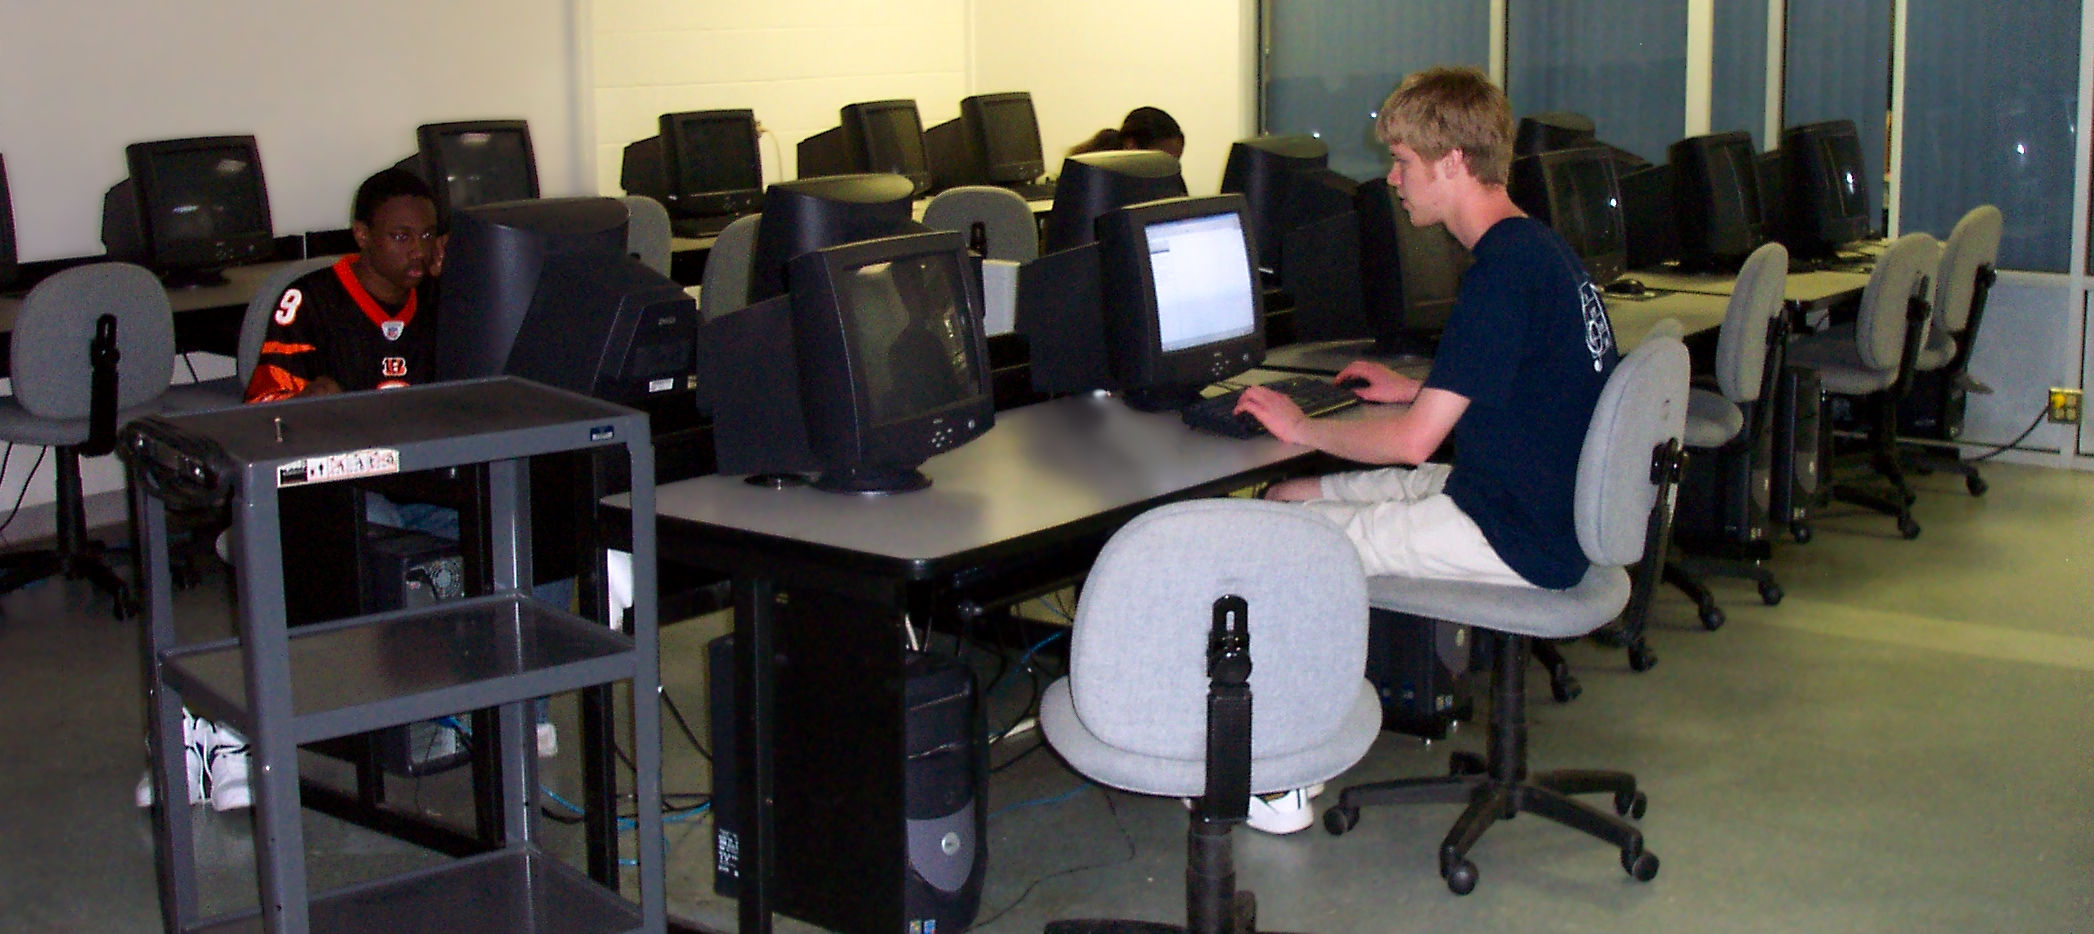
\includegraphics[width=\textwidth]{hayes-20050405-ah208}\\
AH 208 at 4:30 PM on April 5, 2005
\end{center}
\end{frame}


\begin{frame}{My Experience Taking this Course}
\centerline{%
\includegraphics[width=\textwidth, frame, margin=6pt, bgcolor=white]{hayes-2005schedule}}
\end{frame}

\begin{frame}{Passing Data Structures}
  Data Structures is a \emph{marathon}, \textbf{not} a \textit{sprint}.

  \begin{columns}[c]
    \column{0.60\textwidth}
    \begin{itemize}
    \item<2-> Last semester included 24 labs, 3 projects, an ethics paper, and 2 exams.
    \item<3->\emph{Warning:} \textit{The pass rate of a student becoming 3 weeks behind is 0\%}.
    % 2 Weeks is 10\%
    \item<4-> If you are behind, please see me!
    \end{itemize}
  \column{0.30\textwidth}
    \begin{center}%
      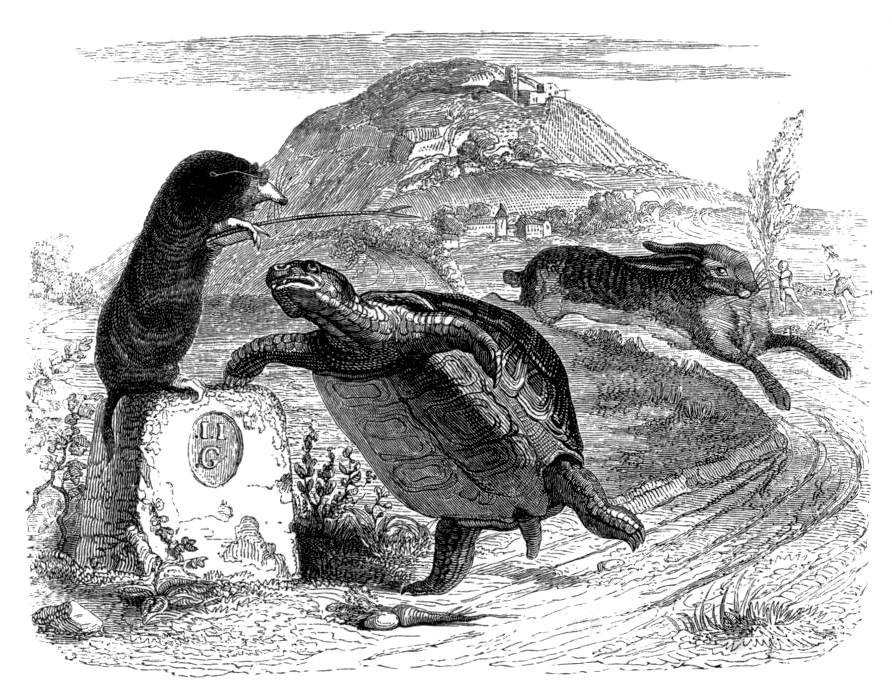
\includegraphics[width=\textwidth]{grandville_tortoise}\\
      \footnotesize{Illustration from the 1855 edition of La Fontaine's Fables}
    \end{center}
  \end{columns}
\end{frame}


\begin{frame}{Passing Data Structures}

    \begin{block}{Advice from a student who passed D.S. and Calc. 2 together while playing football.}
    \begin{itemize}
      \item Do some Data Structure \& Calculus 2 each day.
      \item Do not get behind.
      \item If get stuck, \emph{ensure your code compiles} to get partial credit.
      \item If behind, don't try to catch up; take the 0 and move on.
    \end{itemize}
    \end{block}
\end{frame}

\section{\href{https://csu-cs.github.io/csci-315/syllabus}{Syllabus}}

\begin{frame}{Warning:}
\begin{itemize}
\item Most students consider this class to have the highest workload.
\item This class prepares you for work experience.
\end{itemize}
\end{frame}

\section{Dev. Environment}

%\begin{frame}{}
%\begin{itemize}
%\item git: used as our repository of code, lectures, and assignments
%\item gcc: a compiler toolchain used to translate our C++ programs into machine-executable programs
%\item cxxtest: a test suite to build and automate are testing
%\item make: a tool to simplify building, testing, cleaning, and other utilities
%\item text editor: use to write your programs
%\item bash: our shell/Command Line Interface we use to run our programs
%\item These tools make up our development environment
%\item How is this different than an IDE?
%\end{itemize}
%\end{frame}

\begin{frame}{Unix/Linux Environment}
For this course, you may use any Linux environment.
\begin{itemize}
\item
  I use Ubuntu in the \textit{Windows Subsystem for Linux} (\textbf{WSL}).
\item
  Another good option is \href{https://linuxmint.com/}{Linux Mint} within \href{https://www.virtualbox.org/}{VirtualBox}.\\
  Make sure you \emph{install} Linux.
\item Other options:
  \begin{itemize}
  \item \href{https://linuxmint.com/}{Mint}, \href{https://ubuntu.com}{Ubuntu}, \href{https://getfedora.org/}{Fedora},
    \href{https://www.centos.org/}{CentOS}, etc., should work fine.
  \item macOS: Dual-boot with \href{https://asahilinux.org/}{Asahi Linux}. See \href{https://youtu.be/10thOSWGrpc}{this video} on the setup.
  \item Windows CLI is not compatible with some required tools.
  \item Unix OSs like \href{https://en.wikipedia.org/wiki/Berkeley_Software_Distribution}{BSD} \& \href{https://www.oracle.com/solaris}{Solaris}: I haven't tried, but it should be fine.
  \end{itemize}
\end{itemize}
See the \href{https://csu-cs.github.io/csci-315/guides/setup-overview}{Computer Setup Guide} for more information.
\end{frame}

\begin{frame}{Unix/Linux Environment}
\begin{block}{Setting up WSL with Ubuntu/Debian on Windows 10/11}
  \begin{itemize}
  \item Follow the \href{https://docs.microsoft.com/en-us/windows/wsl/install}{Official Installation Guide} to install Ubuntu 24.04 or later.
  \item For a lab machine, add Ubuntu in WSL from your account (ask for help).
  \end{itemize}
\end{block}
\end{frame}

\begin{frame}{The Windows Subsystem for Linux}

\begin{columns}[c]
\column{0.60\textwidth}
  \begin{itemize}
  \item Our lab has Windows 11 with the Windows Subsystem for Linux \emph{enabled}.
  \item You will need to install Ubuntu on Windows.
  \item Please login with your standard CSCI login.
  \item Install Ubuntu from the Microsoft Store or by running the command: \lstinline[language=bash]{wsl --install -d ubuntu}
  \end{itemize}
\column{0.40\textwidth}
  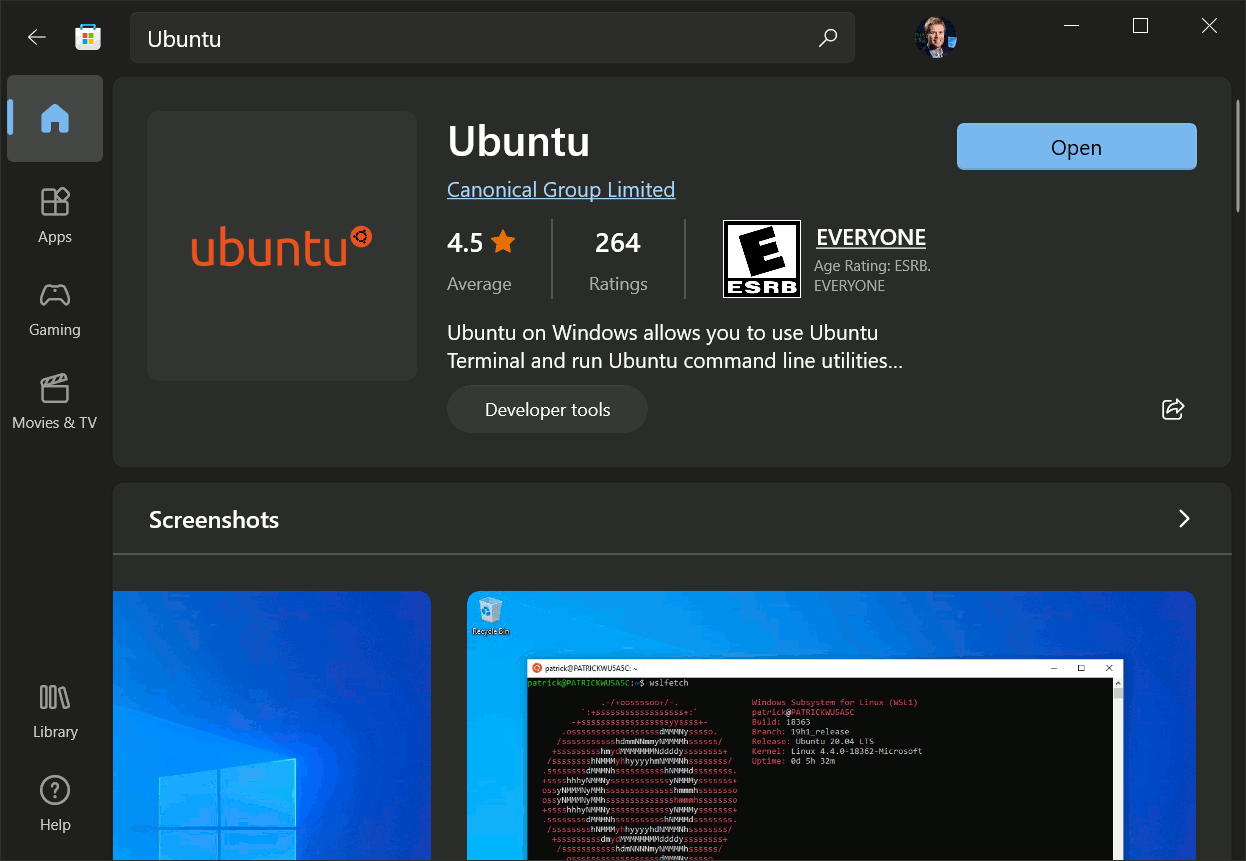
\includegraphics[width=\textwidth]{wsl-ubuntu-install}
\end{columns}
\end{frame}

\begin{frame}{CLI Environment}
  We will be using the Command Line Interface (CLI).
\begin{columns}[T]
\column{0.42\textwidth}
Why?
  \begin{itemize}
  \item It forces you to understand more of what is actually happening.
  \begin{itemize}
  \item Most GUIs are ``paint'' on top of other programs
  \end{itemize}
  \item For many tasks, you can accomplish a lot more in less time. \\
  \end{itemize}
\column{0.50\textwidth}
  \begin{figure}
  \caption{Geeks and repetitive tasks.}
  
\includegraphics[width=\textwidth]{cli-vs-gui}
  \end{figure}
\end{columns}
\end{frame}

\begin{frame}{Terminal}
\begin{itemize}
\item
  The \emph{terminal} (terminal emulator) is a text-only window in a graphical user interface (GUI) that emulates a console.
\item
  It is where we use our CLI.
\item
  Run whatever you want (xterm, LilyTerm, Alacritty, LXTerminal, Extraterm, etc.)!
\end{itemize}
\end{frame}

\begin{frame}{Opening a Terminal}
  \begin{columns}[c]
  \column{0.6\textwidth}
    \begin{itemize}
    \item The terminal window shows a standard prompt.
    \item Prompts display all kinds of information, but they are not part of the commands you are giving to your system.
    \end{itemize}
  \column{0.40\textwidth}
    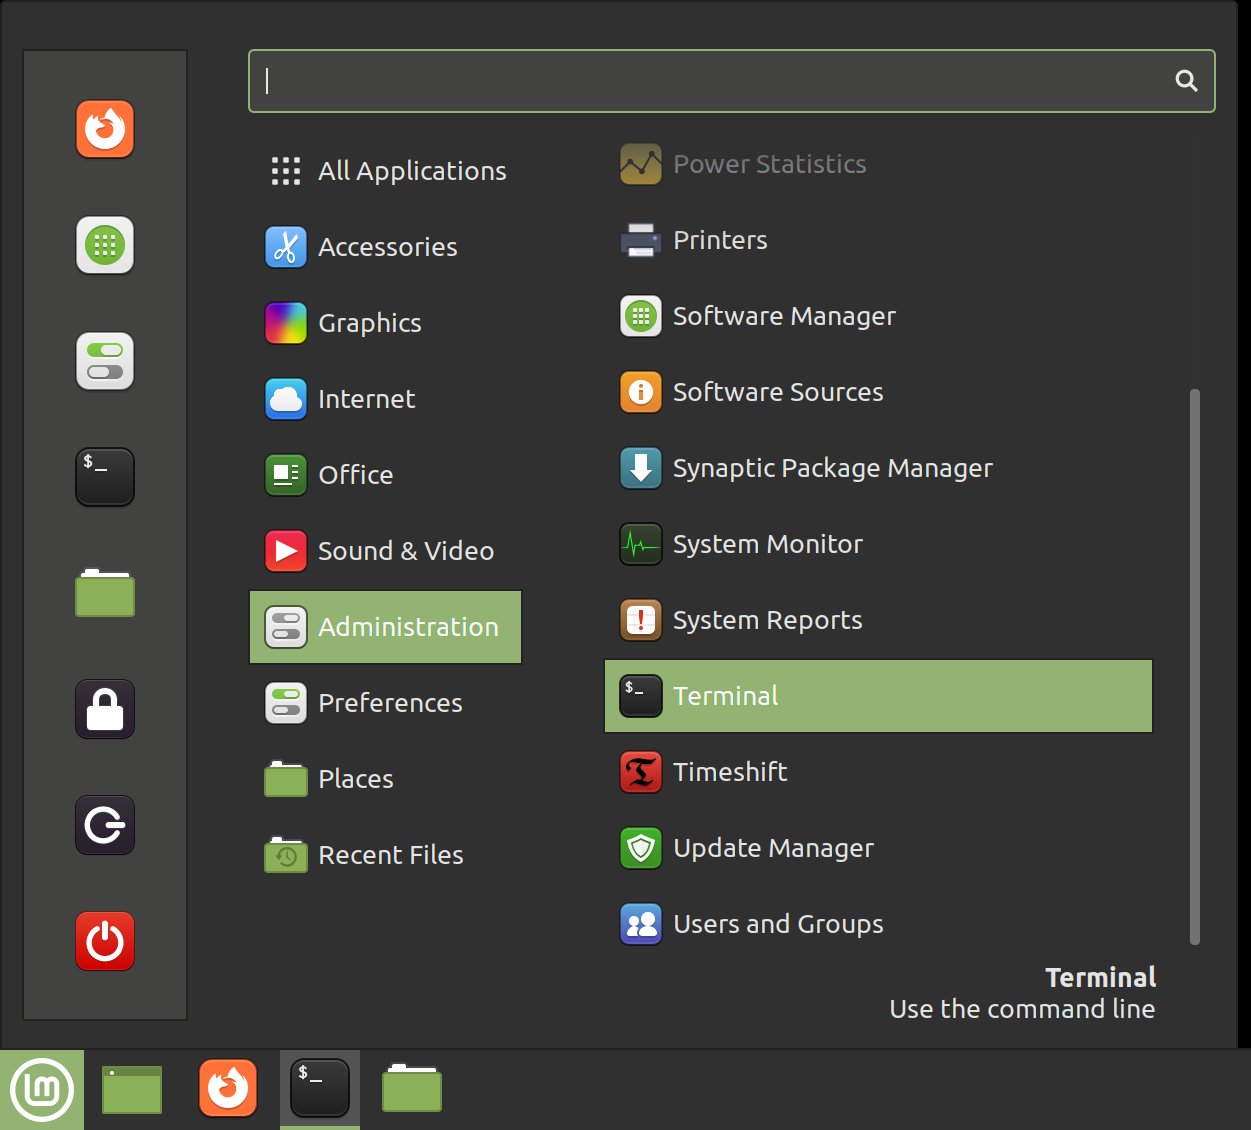
\includegraphics[width=1.0\textwidth]{terminal-open}\\\vspace{0.5em}
    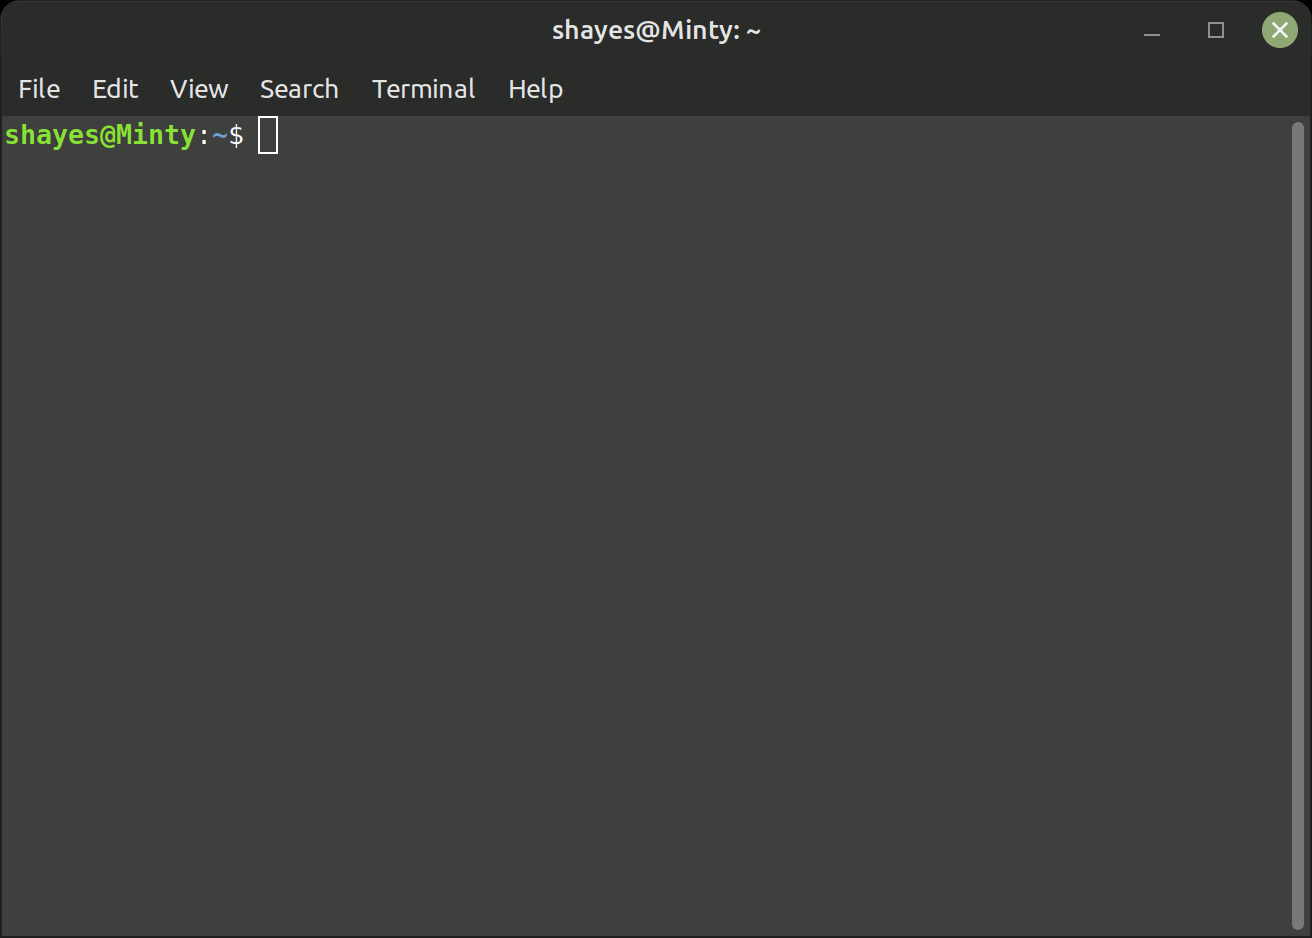
\includegraphics[width=1.0\textwidth,trim={0 600px 0 0},clip]{terminal}
  \end{columns}
  \end{frame}
  
\begin{frame}[fragile]{Install Required Software}
  % \begin{enumerate}
  % \item<+->
    On your Linux box (Mint, Ubuntu, Ubuntu on Windows), install the basic packages for our course.
\begin{lstlisting}[language=bash]
sudo apt update
sudo apt install -y build-essential git valgrind gnuplot
\end{lstlisting}
\end{frame}

\section{Git}

\begin{frame}{Git --- A Version-Control System}
\begin{columns}[T]
\column{0.5\textwidth}
Git:
\begin{itemize}
  \item Developed by \href{https://en.wikipedia.org/wiki/Linus_Torvalds}{Linus Torvalds}.
  \item Very Popular
  \item Open Source and Free!
  \item Just a folder in a directory
  \item Distributed -- every copy (clone) has everything.
\end{itemize}
\column{0.45\textwidth}
\uncover<2->{%
  Other Version-Control Systems:
  \begin{itemize}
    \item Subversion (SVN)
    \item Concurrent Versions System (CVS)
    \item Perforce
    \item Mercurial
  \end{itemize}
}
\end{columns}
\end{frame}

\begin{frame}[fragile]{Other Important Git Settings}
  While you are at it, also store your name and email address:
\begin{lstlisting}[language=bash]
git config --global credential.helper store
git config --global user.name "Your Name"
git config --global user.email "you@student.csuniv.edu"
\end{lstlisting}

The first statement tells git to save your password.\\
Warning: passwords will be saved as plain text on your computer.

\end{frame}

\begin{frame}{Golden 6 of Git}
\begin{description}[commit -m "<message>"]
  \item[\textbf{\texttt{init}}] create a local repository.
  \item[\textbf{\texttt{clone <repo>}}] make a copy of a repository
  \item[\textbf{\texttt{add <file(s)>}}] add one or more files to the staging area (index).
  \item[\textbf{\texttt{commit -m "<message>"}}] save the files permanently in the version history with a message.
  \item[\textbf{\texttt{push}}] sync local repository to a remote repository.
  \item[\textbf{\texttt{pull}}] receive content from a remote repository.
\end{description}
\end{frame}


\section*{GitHub Setup}

\begin{frame}{Lab 0: Github Username}
\begin{center}\Large
  Follow the instructions for Lab 0.
\end{center}
\end{frame}

\begin{frame}{Joining the Class}
  \begin{itemize}
  \item Create a \href{https://github.com/}{GitHub} account (if needed) and log in.
  \item Post your user name to the Blackboard assignment.
  \item You will receive an email to become a collaborator.
  \item Click the email link and join.
  \item Click on the \href{https://github.com/csu-cs/CSCI-315-2026-Spring/}{\texttt{CSCI-315-2026-Spring}} repository.
  \item Click ``Fork''.
  \item Clone your forked repository:\\
  \lstinline{git clone <your repo>}
  \item Let's look through the repository\textellipsis
  \end{itemize}
\end{frame}

\begin{frame}[fragile]{GitHub Personal Access Token}
  Your GitHub password cannot be used to clone your forked repository. Instead, you need to use a different authentication method. GitHub's \href{https://docs.github.com/en/authentication/keeping-your-account-and-data-secure/managing-your-personal-access-tokens}{personal access token} is an easy option. Follow the instructions in the above link to create and use your personal access token.
  \begin{itemize}
    \item I suggest selecting ``No expiration'' for the token expiration.
    \item Select only ``repo'' as the scope of the token.
  \end{itemize}
\end{frame}

\begin{frame}[fragile]{GitHub Personal Access Token}
  \begin{itemize}
    \item When you clone your repository, you will be prompted for your username and password.
    \item Use your GitHub username and the personal access token as the password.
    \item If you are using WSL, you can store your personal access token in the credential helper:
\begin{lstlisting}[language=bash]
git config --global credential.helper store
\end{lstlisting}
    \item This will store your credentials in plain text, so be careful.
  \end{itemize}
\end{frame}

\end{document}